\chapter{Approximating Type Stability Statically}\label{chap:approx}

\lstset{language=julia}

% \paragraph{Plan of attack}
% \begin{enumerate}

% \item
% Inferring type stability versus inferring types

% \item
% Method: Using Julia's built-in type inferencer to approximate type stability.

% \item
% Basic algorithm
% - flowchart, main steps, running example

% \item
% Enumerating concrete subtypes
% -

% Meta: features of the algorithm I'd like to discuss at some point.
% - Corner cases, termination, fuel.
% - Limitations: incompleteness and unsoundness.
% - Relation to Julia subtyping.

% \item
% State space explosion
% due to under-constrained types, e.g.:
% - ''fat'' (i.e. many subtypes) abstract types like Any
% - unbounded existentials
%
% We propose two approaches to fight this problem:
% - run type inference with Any: concrete result means it's stable
% - the types DB idea

% \item 
% Implementation
% - User's API (macro and otherwise)?

% \item
% Evaluation
% - Processing Julia modules: pitfalls and workarounds.
% - Results on 10 popular Julia packages.


% \end{enumerate}

Chapters~\ref{sec:empirical} and~\ref{sec:jules} consider type stability as it
relates to program \emph{execution}: chapter~\ref{sec:empirical} analyzes Julia
VM state after package test suites ran, and chapter~\ref{sec:jules} models a
type-specializing just-in-time compiler that does its main job at the run time.
In this chapter, I set to approximate the property of type stability for
arbitrary Julia code statically, without running the code in question.

\paragraph{Note on Dropping Type Groundedness} It turns out that attempts to
infer type groundedness statically fail fast: this is too low-level of a
notion requiring us to reason on a level of intermediate representation, and at
that level precision gets lost very fast. The good news is that, as we learned
in~\chapref{sec:jules}, type groundedness is enabled by calling type-stable
API, so being able to provide such API should be enough for a careful client.
Therefore, in this chapter we focus on analyzing type stability of methods, and
leave type groundedness off.

\section{Inferring Type Stability versus Inferring Types}

Explaining my method to infer type stability requires a definition for it.
So far, I approached the definition twice: informally
in~\ref{ssect:ts-informal} and formally in~\ref{sec:stability-formal}.
The original informal
definition does not take into account the distinction between concrete and
abstract types: using this loophole, any code can be declared type stable
because it is always possible to ``predict the type of the output'' as \c{Any}.
Building upon the formal definition (that does acknowledge the distinction
between abstract and concrete types)
we provide another informal definition to explain intuitions behind this
chapter.
\begin{definition}[Type Stability, Informally]
  A Julia method is called \emph{type stable} if for any concrete type of the
  input, it is possible to infer a concrete type of the return value.
\end{definition}

A natural idea for inferring type stability in Julia would be to formulate it as
a forward static analysis: being an abstract or concrete type is one bit of
information that has a known value at the input (concrete) and should be
propagated to the output, possibly changing on the way.

To test the static analysis idea, consider a positive example first: the
identity function.
% TODO: there's a weird break in the listing near page break (see PDF)
\begin{lstlisting}
  function id(x)
    x
  end
\end{lstlisting}
%
It is straightforward to infer that, given any concrete input type, the return
value is also concretely typed: the one bit of information carries over to the
result in one step.

Another example, the increment function, shows that the task becomes unwieldy fast.
%
\begin{lstlisting}
  function inc(x)
    x + 1
  end
\end{lstlisting}
%
Concreteness of the result returned by \c{inc} depends on the same property of
the result of the call to \c{+}. In turn, the property of the return type of
\c{+} depends on which \c{+} method Julia will dispatch to at the run time.
There are about two hundreds method implementations of \c{+} in the standard
library alone, and packages add more. Some of those methods are type stable
(e.g. \c{+(::Int64,::Int64)}), and some of them not (e.g.
\lstinline|+(::Rational{Bool},::Rational{Bool}|)
\footnote{%
  The reason for the
  \c{+(::Rational\{Bool\},::Rational\{Bool\})} method to be not type
  stable is not important, but in a nutshell, Julia has made a questionable
  design decision about the return type of \c{{+}(::Bool,::Bool)}, which in the
  current implementation is \c{Int}
  (see discussion \url{https://github.com/JuliaLang/julia/issues/19168}),
  and when adding two rational numbers with boolean components, depending on the
  values of the summands, you get back either \c{Rational\{Bool\}} or
  \c{Rational\{Int\}}.}
).
Therefore,
to infer the property of interest, in general,
we need to predict which methods are selected at the run time.

The \c{inc} example shows that inferring type stability of Julia code
requires
reasoning about which methods will be called at the run time, which, in a
language with dynamic dispatch, leads
to reasoning about the \emph{types} of intermediate values, rather than only
the concreteness bit. But if we had a tool to compute typing information
beforehand, we would not need to build a special purpose analysis for type
stability: it suffices to ask the tool for the type of the return value and
check if that type is concrete. The observation of interactions between type
stability and type inference can be formulated as the following conjecture.

\begin{conjecture}
  Inferring type stability of a Julia method statically is no easier than doing type
  inference over that method.
\end{conjecture}

A full type inference algorithm would be enough for checking type stability of
Julia code. Should we build one from scratch? There are two reasons to not
avoid this path.
\begin{enumerate}

  \item It is not clear that typing Julia without changing anything in the
  language can yield a meaningful result (more on this
  see~\cite{Chung23}).

  \item Julia already has a type inference engine built in. We modelled this
        engine as a black box in~\chapref{chap:jules}. If we end up with a
        custom algorithm to infer types and analyze type stability based on it,
        our results may diverge from Julia's. This would be of limited usage for
        Julia users.
\end{enumerate}

\section{An Algorithm To Approximate Type Stability}%
\label{sec:algo}

If our predictions for type stability are to align with the Julia
implementation, our analysis should closely model what happens at the run time,
as described in~\chapref{chap:jules}. The type-specializing JIT-compiler
from~\chapref{chap:jules} makes optimization decisions based on \emph{concrete
  input types} with the help of Julia's type inference engine. Our algorithm for
approximating these decisions statically considers all (or as many as possible,
see~\secref{sec:term}) allowed concrete input types of a method.
\figref{fig:infer-ts} describes this algorithm at a high level.

\begin{figure}
  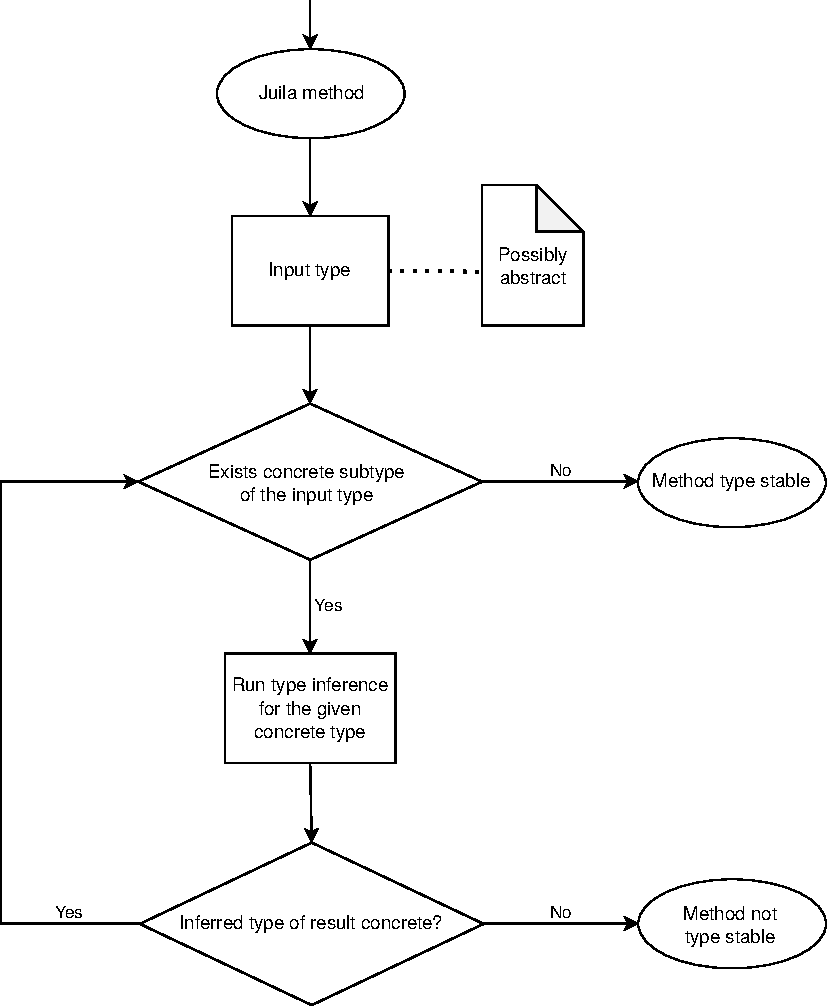
\includegraphics{figs/infer-ts.pdf}
  \caption{Inferring type stability of a Juila method}%
  \label{fig:infer-ts}
\end{figure}


Let us consider every step of the algorithm described
on~\figref{fig:infer-ts} and show its meaning using an example.
The list below also assigns the numbers to each step in our algorithm.
\begin{enumerate}

  \item The input of the algorithm is a Julia method. Methods in Julia are
  represented by runtime objects of type \c{Method} and can be manipulated as
  all other objects (e.g. stored in collections, responding to field accesses, etc.).

  For example, consider the \c{length} method from the Julia's standard library. We can
  get the corresponding \c{Method} object using the standard \c{@which} macro
  applied to an application of the \c{length} method. This can be done in the
  Julia REPL (signified by the \texttt{julia>} prefix).

\begin{minipage}{.92\textwidth}
\begin{lstlisting}[style=jterm]
  julia> @which length([1,2,3])
  length(a::Array) in Base at array.jl:215
\end{lstlisting}
\end{minipage}

  The output shows that the given \c{length}-call will dispatch to the
  method defined in the \texttt{Base} module (Julia-speak for the standard
  library). The output also shows the location of the method in the
  standard library and, most importantly for us, the signature of the
  method. In fact, what we see here is a pretty-printed representation of
  the \c{Method} object representing a particular Julia method.

  \item The first task of the algorithm is to get the input type of the given
  method. This is possible through querying the \c{sig} field of the method object.

  Building on the example above, we can get the signature of the \c{length}
  method as follows:

\begin{minipage}{.92\textwidth}
\begin{lstlisting}[style=jterm]
  julia> m = @which length([1,2,3]);

  julia> m.sig
  Tuple{typeof(length), Array}
\end{lstlisting}
\end{minipage}

  A signature of a method will usually have the special singleton function
  type (\c{typeof(...)}) as the first component, and the rest is (easy to
  convert to) the type of the input --- an $n$-tuple. In this example, the type of
  the input is 1-tuple, consisting of the existential array type
  \c{Array\{T, N\}\ where T where N} abbreviated simply as \c{Array}\footnote{%
A user can always look under the abbreviation using the \c{dump} function.
%:
% \begin{lstlisting}[language=julia,style=jterm]
%   julia> dump(Array)
%   UnionAll
%     var: TypeVar
%       name: Symbol T
%       lb: Union{}
%       ub: Any
%     body: UnionAll
%       var: TypeVar
%         name: Symbol N
%         lb: Union{}
%         ub: Any
%       body: Array{T, N} <: DenseArray{T, N}
% \end{lstlisting}
}.

  \item The input type can be either concrete, which, in Julia, means there may
  be no proper subtypes of that type, or abstract. Still, the choice on the
  step 3 will enter the loop at least once, because if the input type is
  concrete, the check holds once trivially (e.g.\ there is exactly one concrete
  subtype of the concrete type \c{Int} --- it is \c{Int} itself).

  If the input type is abstract, we need a subprocess enumerating all concrete
  subtypes of it. We discuss an implementation for this below but it suffices to
  treat is as a black box for now. % TODO: ref to subtyping section?

  In the case of the \c{length} method, the input type, \c{Array}, is abstract
  because it is an existential type.

  \item Running type inference for a given method and a given concrete input
  type is done through calling the Julia's standard \c{code\_typed} function.
  The only issue with the function is that it expects a function object as the
  part of the input, not a method object. But getting from a method to the
  corresponding function is possible using the signature field discussed above,
  and, in particular, the singleton function type living in the first component
  of the \c{sig} field: accessing the single function object using the function
  type is possible via the \c{instance} field.

  Running type inference for the \c{length} method and the concrete input type
  \c{Array\{1, Float64\}} could be done as follows:

\begin{minipage}{.92\textwidth}
% \begin{verbatim}
\begin{lstlisting}[style=jterm]
  julia> code_typed(m.sig.parameters[1].instance,
                    (Array{1, Float64},),
                    optimize=false)
  1-element Vector{Any}:
   CodeInfo(
  1 - %1 = Base.arraylen(a)::Int64
  +--      return %1
  ) => Int64
\end{lstlisting}
% \end{verbatim}
\end{minipage}

  \item In the running example and for the input type \c{Array\{1, Float64\}}
  the type inferencer is able to deduce that the return type of \c{length}
  called with the given input type is \c{Int64}, which is a concrete type
  according to the standard Julia's \c{isconcretetype} predicate.
  Following the second decision element on \figref{fig:infer-ts}, we get back to
  the start of the loop and try another concrete subtype of the input type,
  if there is any.
\end{enumerate}

There are two main auxiliary procedures that the algorithm relies on: enumeration of
concrete subtypes of a given input type and type inference over a method with the
given input type. The latter can be fully outsourced to Julia itself, while the
former requires separate consideration.

\subsection{Enumerating Concrete Subtypes}%
\label{sec:approx:enu}

\subsubsection{Nominal Hierarchy (Julia's \c{subtypes} method)}

In Step 3 of the algorithm (\figref{fig:infer-ts}), we need to generate a
concrete subtype of the input type. This task does not have a direct
implementation in Julia's standard library. The closest counterpart that Julia
provides is the \c{subtypes} method to query declared subtypes of a given
nominal type. For example,
\begin{figure}[h]
\begin{minipage}{.49\textwidth}
\begin{lstlisting}[style=jterm]
julia> subtypes(Signed)
6-element Vector{Any}:
 BigInt
 Int128
 Int16
 Int32
 Int64
 Int8
\end{lstlisting}
\end{minipage}
~
\begin{minipage}{.49\textwidth}
\begin{lstlisting}[style=jterm]
julia> subtypes(AbstractSet)
5-element Vector{Any}:
 Base.IdSet
 Base.KeySet
 BitSet
 Set
 Test.GenericSet

\end{lstlisting}
\end{minipage}
\end{figure}

The challenge here is that the subtype relation in Julia is richer than the
nominal type hierarchy. For example, if a method declares the type of its input
as
\begin{lstlisting}
  Union{AbstractSet, AbstractRange}
\end{lstlisting}
then the method can be called with an argument of type \c{Set\{Int\}}, and,
therefore, we should be able to discover such a type following the algorithm
on~\figref{fig:infer-ts}. It is not possible with the \c{subtype} method alone:
\begin{lstlisting}[style=jterm]
  julia> subtypes(Union{AbstractSet, AbstractRange})
  Type[]
\end{lstlisting}
which means that from \c{subtypes}' point of view this type has no subtypes (the query
returns an empty array of elements of the type \c{Type}). Therefore, structural
types like unions, tuples and existential types need a special treatment.

The \c{subtypes} method does not cover the whole subtyping relation not only
because it cannot work with structural types but also because it only knows
about direct declared subtypes: in the subtype chain \c{Int <: Signed <:
Integer}, \c{subtypes} only knows about \c{Int <: Signed} and \c{Signed <:
Integer} but not about \c{Int <: Integer}. Thus, we have to build
the transitive closure manually.

In the following section, I show how to generalize the \c{subtypes} method
for all Julia types. After that I discuss how to iterate the general version to
get to the concrete types.

\subsubsection{Enumerating Direct Subtypes}

Our goal is to define a general utility generating direct subtypes of a given
type, which we call \c{direct_subtypes}.
% \begin{lstlisting}
%   const JlType = Any   # type synonym
%   function direct_subtypes(t :: JlType) :: Vector{JlType} ...
% \end{lstlisting}
We do case analysis on the existing Julia kinds and express it as methods
of the \c{direct_subtypes} function. The implementation largely follows from the
description of Julia's subtyping relation given in~\cite{oopsla18b}.

The \c{direct_subtypes} utility can be defined, for the most part, via multiple dispatch
using Julia's kind system.
The only special sort of types that does not have a dedicated kind is tuple types.
purpose. In particular, although tuple types fall under the datatype kind,
the standard \c{subtypes} method cannot help with tuple types as much as it can with user-defined datatypes.
For example:
both \c{Integer} and \c{Tuple\{Integer, Integer\}} are datatypes, but
\c{subtypes} returns an empty array of types for the latter.

%
% good for the Background section, perhaps?
% Generally, every Julia type is
% either a union type (kind \c{Union}), an existential type (kind \c{UnoinAll}) or
% a datatype (kind \c{DataType}), for example:
% \begin{lstlisting}[style=jterm]
%   julia> Union{Int, String} isa Union
%   true
%   julia> Vector isa UnionAll
%   true
%   julia> Int isa DataType
%   true
% \end{lstlisting}

% Overall,
% some special types, notably tuple types, fall under the datatype kind. Still,
% existing kinds other than \c{DataType}, are useful.

\begin{description}

  \item[Union Types]
        Unions in Julia has the kind \c{Union} and a form of \c{Union\{A,B,C\}}
        with arbitrary number of arguments \c{A, B, C}.
        Direct subtypes of \c{Union\{A,B,C\}} is the following list of types: \c{[A,B,C]}.

  \item[Existential Types]
        Existential types in Julia has the kind \c{UnionAll} and a form of
        \c{Vector{T} where T} commonly abbreviated as \c{Vector}. Every
        \c{where}-bound type variable has associated upper and lower bounds with
        default values \c{Any} and \c{Union\{\}} (the top and bottom types),
        respectively. Direct subtypes of an existential type is all
        instantiations of its variable allowed by the bounds. In particular, we
        need to compute all subtypes of the upper bound, filter out those not
        satisfying the lower bound, and use the resulting set of types to
        instatiate the variable with.

        For example, consider the \c{Vector\{T\} where T<:Signed} type.
        All subtypes (not only direct or concrete) of \c{Signed} are: \c{BigInt, Int128, Int16, Int32, Int64, Int8}. Therefore, all direct subtypes of the vector type in question are:

\begin{minipage}{.92\textwidth}
        \begin{lstlisting}
Vector{BigInt}
Vector{Int128}
Vector{Int16}
Vector{Int32}
Vector{Int64}
Vector{Int8}
        \end{lstlisting}
\end{minipage}

  \item[Datatypes]
        In general, non-parametric nominal types defined using the \c{primitive} (e.g. \c{Int64}) or
        \c{struct} (e.g. \c{Pair}) qualifiers,  can be processed
        using the \c{subtypes} method (see examples in the previous section).%:
        These also include fully-instantiated parametric types
        (e.g. \c{AbstractSet\{Int\}}).

  \item[Tuple Types]
        Tuples play a key role in method dispatch because methods with
        more than one argument have a tuple input type. As the \c{subtypes} method
        cannot work with tuples (for any input tuple, it returns an empty
        array), we need to manually unfold tuple types using the following rule
        \begin{itemize}
          \item direct subtypes of the 0-tuple type is an empty set;
          \item direct subtypes of a 1-tuple type are the direct subtypes of its
          single type argument;
          \item direct subtypes of an $n$-tuple type are a Cartesian product of
          direct subtypes of its first component and direct subtypes of the last
          $n-1$ components.

          For example, for an abstract type \c{A} with exactly two declared
          subtypes \c{B} and \c{C}, the set of direct subtypes of
          \c{Tuple\{A,A\}} is

\begin{minipage}{.9\textwidth}
        \begin{lstlisting}
Tuple{B,B}
Tuple{B,C}
Tuple{C,B}
Tuple{C,C}
        \end{lstlisting}
\end{minipage}

        \end{itemize}

        % % TODO: This section is to be moved to the discussion of state space size.
        % % General idea (which is not yet expressed in this text) is that we
        % probably don't want to enumerate all singleton types.
  % \item[Special Singleton Types]
  %       In Julia, every type with a single instance is called singleton type.
  %       If it is a regular user-defined type (like \c{Val} from the standard
  %       library), then it can be processed using the general strategy described
  %       above (as a datatype or an existential type, depending on its form).
  %       But two
  %       kinds of Julia values has special singleton types:
  %       \begin{itemize}
  %         \item Every function has a dedicated \c{typeof}-type (e.g. the
  %         function \c{sum} has the type \c{typeof(sum)}). The \c{typeof}-types
  %         are concrete and therefore have an empty set of proper direct
  %         subtypes. There is a common supertype for all function types called
  %         \c{Function}. It does not
  %         \item Type objects have \c{Type{T}} types (e.g. \c{Int} has the
  %         \c{Type\{Int\}} type). These types
  %       \end{itemize}
  %       primitive values can be used as arguments of
  %       parametric types (e.g. )

\end{description}

\subsection{Termination}%
\label{sec:term}

It is clear that the algorithm does not terminate for some inputs. Consider the
\c{length} example: its input type is the existential \c{Array} type, which
means that possible concrete input types may be:
\begin{itemize}

  \item \c{Array\{1, Int\}}
  \item \c{Array\{1, Array\{1, Int\}\}}
  \item \c{Array\{1, Array\{1, Array\{1, Int\}\}\}}
  \item etc.
\end{itemize}

The issue of termination is close to another one: a search space blow up.
In the standard library alone, there are over five hundreds immediate subtypes
of \c{Any} and every concrete subtype of those can be used to instantiate the
\c{Array} type when inferring type stability of \c{length}. Although finite, this
space can be simply too large to exhaust in a reasonable time.

Our intention is to develop certain heuristics to perform an early termination
of the algorithm. The simplest heuristic of this sort is to employ a fuel
parameter that gives an arbitrary upper bound for the number of steps we are
allowed to perform before we give up.

\section{Evaluation}%
\label{sec:approx:eval}

In \chapref{chap:empirical} I analyzed type stability of a corpus of open-source
Julia packages dynamically via executing test suites of the packages and
inspecting the resulting method instances collected from the internal state of
the virtual machine. Here, I run the algorithm from \secref{sec:algo} to
statically infer type stability of the same packages and match the
results.
